\documentclass{article}

\usepackage{bounds}
\usepackage{mcode} 



\newcommand\R{{\ensuremath{\mathbb{R}}}}                  % Real numbers
\newcommand\N{{\ensuremath{\mathbb{N}}}}                  % Natural numbers
\newcommand\Z{{\ensuremath{\mathbb{Z}}}}                  % Integers
\newcommand\C{{\ensuremath{\mathbb{C}}}}                  % Complex numbers


\newcommand\Prob[1]{{\ensuremath{\mathbb{P}\left(#1\right)}}}        % Probability
\newcommand\ExV[1]{{\ensuremath{\mathbb{E}\left[#1\right]}}}         % Expected value
\newcommand\var[1]{{\ensuremath{\mathbb{\text{var}}\left(#1\right)}}}         % Variance
\newcommand\cov[1]{{\ensuremath{\mathbb{\text{cov}}\left(#1\right)}}}         % Covariance
\newcommand\bigO[1]{{\ensuremath{\mathcal{O}\left(#1\right)}}}       % Big O operator
\newcommand\spec[1]{{\ensuremath{\text{spec}\left(#1\right)}}}         % spectrum

\newcommand\sizeS{{\ensuremath{l}}}

% Binary operators
\newcommand{\defeq}{\ensuremath{\vcentcolon=}}            % :=
\newcommand{\eqdef}{\ensuremath{=\vcentcolon}}            % =:

\newcommand{\gmrestol}{\ensuremath{\epsilon_{\textsc{gmres}}}}   % GMRES tolerance
\newcommand{\gmresiter}{\ensuremath{N_{\textsc{gmres}}}}         % number of GMRES iterations
\newcommand{\conditionN}{\ensuremath{\kappa}}                       % condition number matrix

% Theorems and lemmas
\newtheorem{theorem}{Theorem}[section]
\newtheorem{lemma}{Lemma}[section]
\newtheorem{proposition}{Proposition}[section]
\newtheorem{corollary}{Corollary}[section]
\newtheorem{definition}{Definition}[section]




\title{Project Template}
\author{Mariana Martínez Aguilar \\ \small{Professor: Laura Grigori}}
\date{December 2024}

\begin{document}
\pagestyle{fancy}
\maketitle


\begin{abstract} %<<<
This is optional, an abstract is just a small summary of the important things in a project. Makes people interested in what they're about to read.
\end{abstract} %>>>

\section{Introduction}

To learn how to write mathematical texts you can refer to Nick Higham's book \href{https://epubs.siam.org/doi/book/10.1137/1.9780898719550}{\say{Handbook of Writing for the Mathematical Sciences}}.

An example of a centered but unnumbered equation

\[ (1 - \varepsilon)\| A x \|_2 \leq \| \Omega A x \|_2 \leq (1 + \varepsilon)\|Ax\|_2.  \]

An example of a lemma

\begin{lemma}[Johnson-Lindenstrauss]
    Given $\varepsilon \in (0, 1)$, a set $X$ of $n$ points in $\R^{m}$, i.e. $X \in \R^{m \times n}$, and an integer $l > 8\log(n)/\varepsilon^{2}$, there is a linear map $f: \R^{m} \to \R^{l}$ such that
    \[ (1 - \varepsilon)\| x - y \|_2 \leq \| f(x) - f(y) \|_2 \leq (1 + \varepsilon) \| x - y \|_2 \]
    for all $x, y \in X$.
\end{lemma}


\subsection{Subsection 1}

To cite from the bibliography you can use this command \cite{tropp_improved_2011}. If you need to cite more than one paper you can put them together \cite{cartis_hashing_2021, chenakkod_optimal_2024, nelson_osnap_2012, nelson_lower_2013}.

An example of a definition. 

\begin{definition}[Leverage scores homogenizers (LSH)]
\label{def: Leverage scores homogenizers (LSH)}
    Let $V \in \R^{m \times n}$ be an orthogonal matrix such that $m \geq n$. A matrix $\hat{H} \in \R^{r \times m}$ with $ m \geq r \geq n$ is called a leverage scores homogenizer (LSH) if the preconditioned matrix $U = \hat{H}V$ satisfies the following properties
    \begin{enumerate}
        \item $\ExV{U^{\top}U} = I_{n \times n}$
        \item $\ExV{U} = 0$, $\ExV{U_{ij}^{2}} = \frac{1}{r}$
        \item Let $L_{U}(\delta)$ be a deterministic function that only depends on the size of $U$ and on $\delta$, then $\Prob{ \| e_{j}^{\top} U \|_2 \leq L_{U}(\delta) } \geq 1 - \delta$ for all $j = 1, ..., r$ i.e. $\hat{H}$ homogenizes the leverage scores of $V$ w.h.p.
        \item We know $\varphi(r, m)$ such that $\|Ux\|_2 \leq \varphi(r, m) \|x\|_2$ (deterministic bound)
    \end{enumerate}
\end{definition} 

Example of a theorem.

\begin{theorem}[Some theorem]
\label{theorem: Some theorem}
    Epsilon subspace embeddings are useful.
\end{theorem}

To prove something.

\begin{proof}
    Exercise left to the reader.
\end{proof}

To reference a theorem or lemma use \cref{theorem: Some theorem}. An example of a corollary.

\begin{corollary}[A corollary]
    \label{corollary: A corollary}
    Math things.
\end{corollary}


\subsection{Another subsection}
 
To insert an image right here use the [H] option.

\begin{figure}[H]
    \centering
    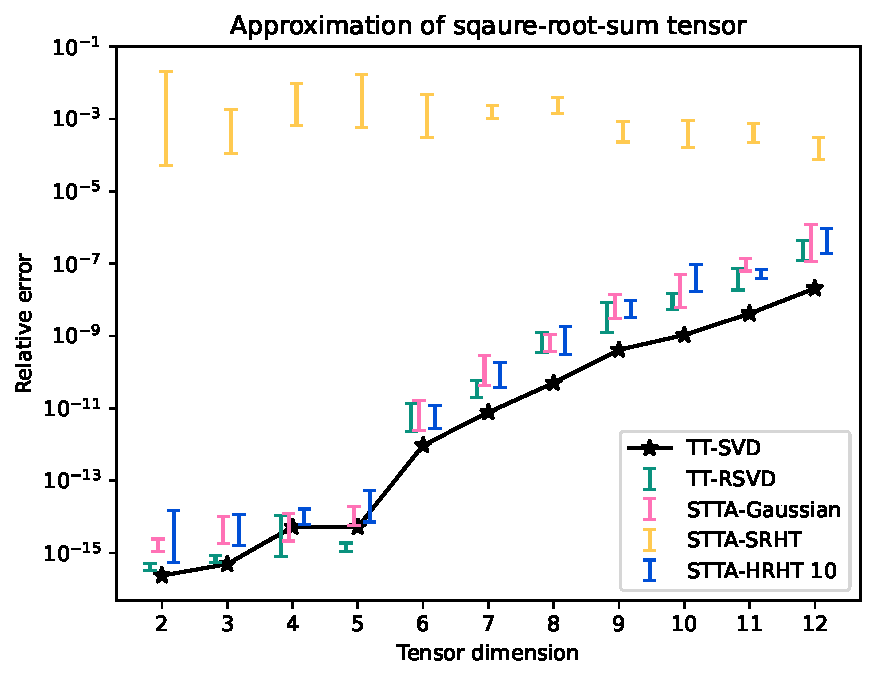
\includegraphics[width=0.8\linewidth]{Images/C_sqrt_sum_d.pdf}
    \caption{Different methods applied to tensor train rounding}
    \label{fig:methods tt rounding}
\end{figure}

This option also works with subfigures.

\begin{figure}[H]
     \centering
     \begin{subfigure}[b]{0.8\textwidth}
         \centering
         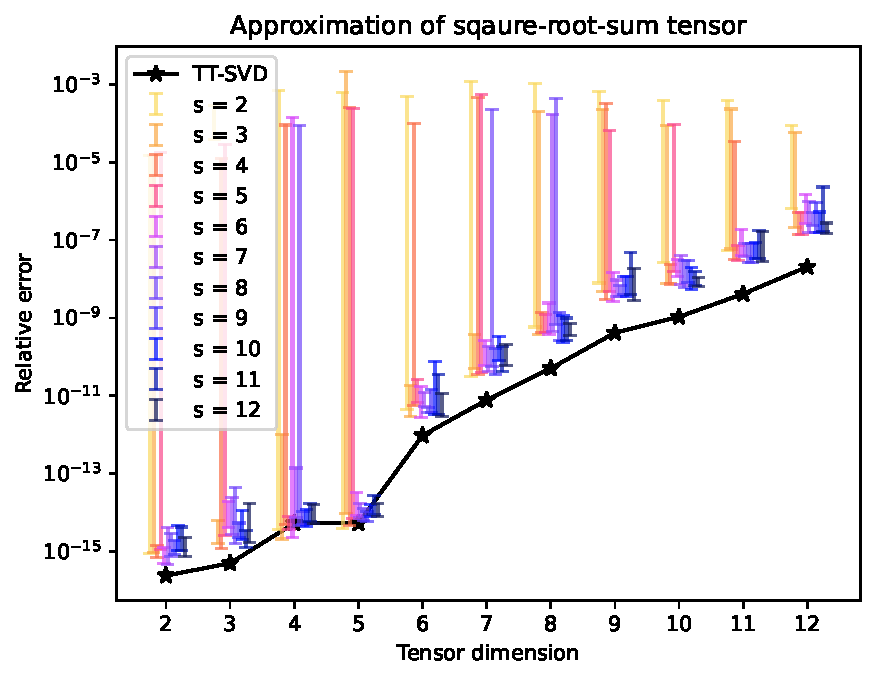
\includegraphics[width=\textwidth]{Images/Cs_sqrt_sum_d.pdf}
         \caption{Sample standard deviation for different $s$}
         \label{fig:error bars s tt rounding}
     \end{subfigure}
     \hfill
     \begin{subfigure}[b]{0.8\textwidth}
         \centering
         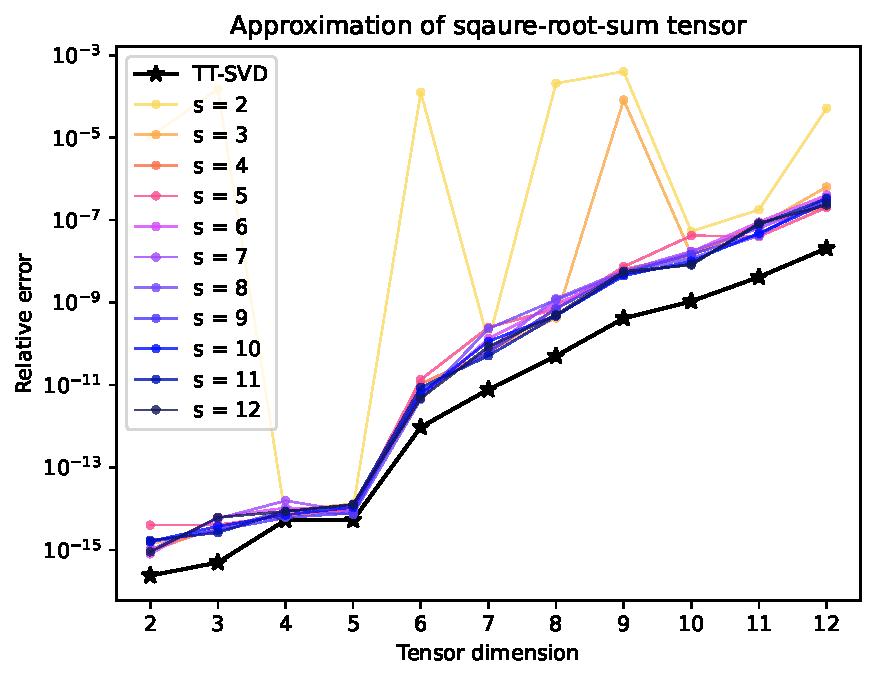
\includegraphics[width=\textwidth]{Images/CsMed_sqrt_sum_d.pdf}
         \caption{Median errors for different. $s$}
         \label{fig:med errors s tt rounding}
     \end{subfigure}
     \caption{Comparison different sizes of $s$}
     \label{fig: errors srht tt rounding}
\end{figure}



\section{Pseudocode}

An example of pseudocode in a very simple format. The packages used are in the .sty file.

\begin{algorithm}
\caption{RQRCP}\label{RQRCP}
\begin{algorithmic}
\Input $A \in \R^{m \times n}$, $\Omega \in \R^{l \times m}$, $k$ $l > k$
\Output $I_{02}$, indices of the columns of $A$ from which to build the low rank approximation
\State Compute $B = \Omega A$, $B \in \R^{l \times n}$.
\State Compute $k$ steps of QRCP on $B$ and select $k$ columns.
\State Return $k$ selected columns, with indices saved in $I_{02}$.
\end{algorithmic}
\end{algorithm}

\section{Code}

You should upload your code as a separate file but this is an option just in case there is a moment where you need to input code as text. 

\lstinputlisting{Code/exercise1.py}


\bibliographystyle{plain}
\bibliography{template}

\appendix
\section{An example of an appendix}

Things written in the appendix are considered to be optional for the reader. Your text should be self contained and the appendix should only include extra information.


\section{An example of another appendix}



\end{document}
